\chapter{Healthcare utilisation: the cost of invisibility}
\label{ch:ch7}

The preceding chapters established that the Italian over-65 population partitions into five distinct profiles and that one of them --- Moderate Isolated ($n = 639$; 26.9\% of the sample) --- combines adequate objective health with an extreme deficit of social integration. This chapter tests whether that invisibility translates into measurable differences in how the health system is used. The finding is specific: the Moderate Isolated cohort systematically under-uses \emph{discretionary} and \emph{prevention-facing} care (doctor visits, specialist contacts, dentist) compared with the matched Traditional Social profile, while the gap on forgone care for cost reasons and on hospital-stay length is statistically indistinguishable from zero. Read jointly, these two patterns support an interpretation of the social network as \emph{navigational capital} for accessing the healthcare system, rather than as a volumetric filter against unmet need.

\section{Data and merge}
\label{sec:ch7-merge}

The analytical dataset is constructed by merging the cluster assignments of Chapters~\ref{ch:ch4} and~\ref{ch:ch5} with SHARE's Healthcare (HC) module. The Italian merge retains $n = 2{,}378$ respondents (100\% match rate); the Swedish merge retains $n = 1{,}787$ respondents (100\%). The outcome indicators refer to the twelve months preceding the SHARE W9 interview and include doctor and specialist visits, general-practitioner contacts, dentist contacts, hospitalisation (any, and nights), and self-reported forgone care because of cost.

\section{The isolation paradox: Moderate Isolated vs Traditional Social (Italy)}
\label{sec:ch7-paradox}

The empirical core of this chapter is the contrast between the Moderate Isolated profile ($n = 639$; CASP $= 36.8$; loneliness $= 3.6$; social-network indicators visibly below the sample mean) and the Traditional Social profile ($n = 184$; CASP $= 38.5$; comparable subjective well-being but strong social integration). Under the assumption that the two profiles experience comparable clinical conditions --- an assumption supported by the similar CASP, loneliness, hope and life-satisfaction values in Table~\ref{tab:ch4-profiles} --- any difference in healthcare utilisation between them is attributable to social factors, not to differences in underlying need.

Table~\ref{tab:ch7-isolati-sociali} reports the mean values of six healthcare indicators for the two profiles, the Moderate-minus-Social gap, the Welch's $t$-test statistic, and the associated $p$-value.

\begin{table}[ht]
  \centering
  \caption{Healthcare utilisation, Moderate Isolated vs Traditional Social (Italy).}
  \label{tab:ch7-isolati-sociali}
  \small
  \begin{tabular}{@{}lrrrrl@{}}
    \toprule
    \textbf{Indicator (12m)} & \textbf{Isolated} & \textbf{Social} & \textbf{Gap} & \textbf{$p$} & \textbf{Sig.}\\
    \midrule
    Doctor visits            &  4.61 &  6.20 & $-1.58$  & $.001$  & $**$\\
    GP contacts              &  4.19 &  4.37 & $-0.18$  & $.602$  & ns\\
    Specialist contacts      &  1.08 &  2.02 & $-0.94$  & $<.001$ & $***$\\
    Dentist (\%)             & 20.97 & 47.83 & $-26.86$ & $<.001$ & $***$\\
    Forgone care for cost (\%)&  5.79 &  5.43 & $+0.36$  & $.998$  & ns\\
    Nights in hospital       &  6.64 &  8.67 & $-2.02$  & $.473$  & ns\\
    \bottomrule
  \end{tabular}
  \par\smallskip
  \footnotesize \emph{Note.} Welch's $t$-test. Binary outcomes (Dentist, Forgone care) tested via proportion test. Values reported in percentage points for binary outcomes. Figures available in Figure~\ref{fig:ch7-isolati-sociali}.
\end{table}

\begin{figure}[ht]
  \centering
  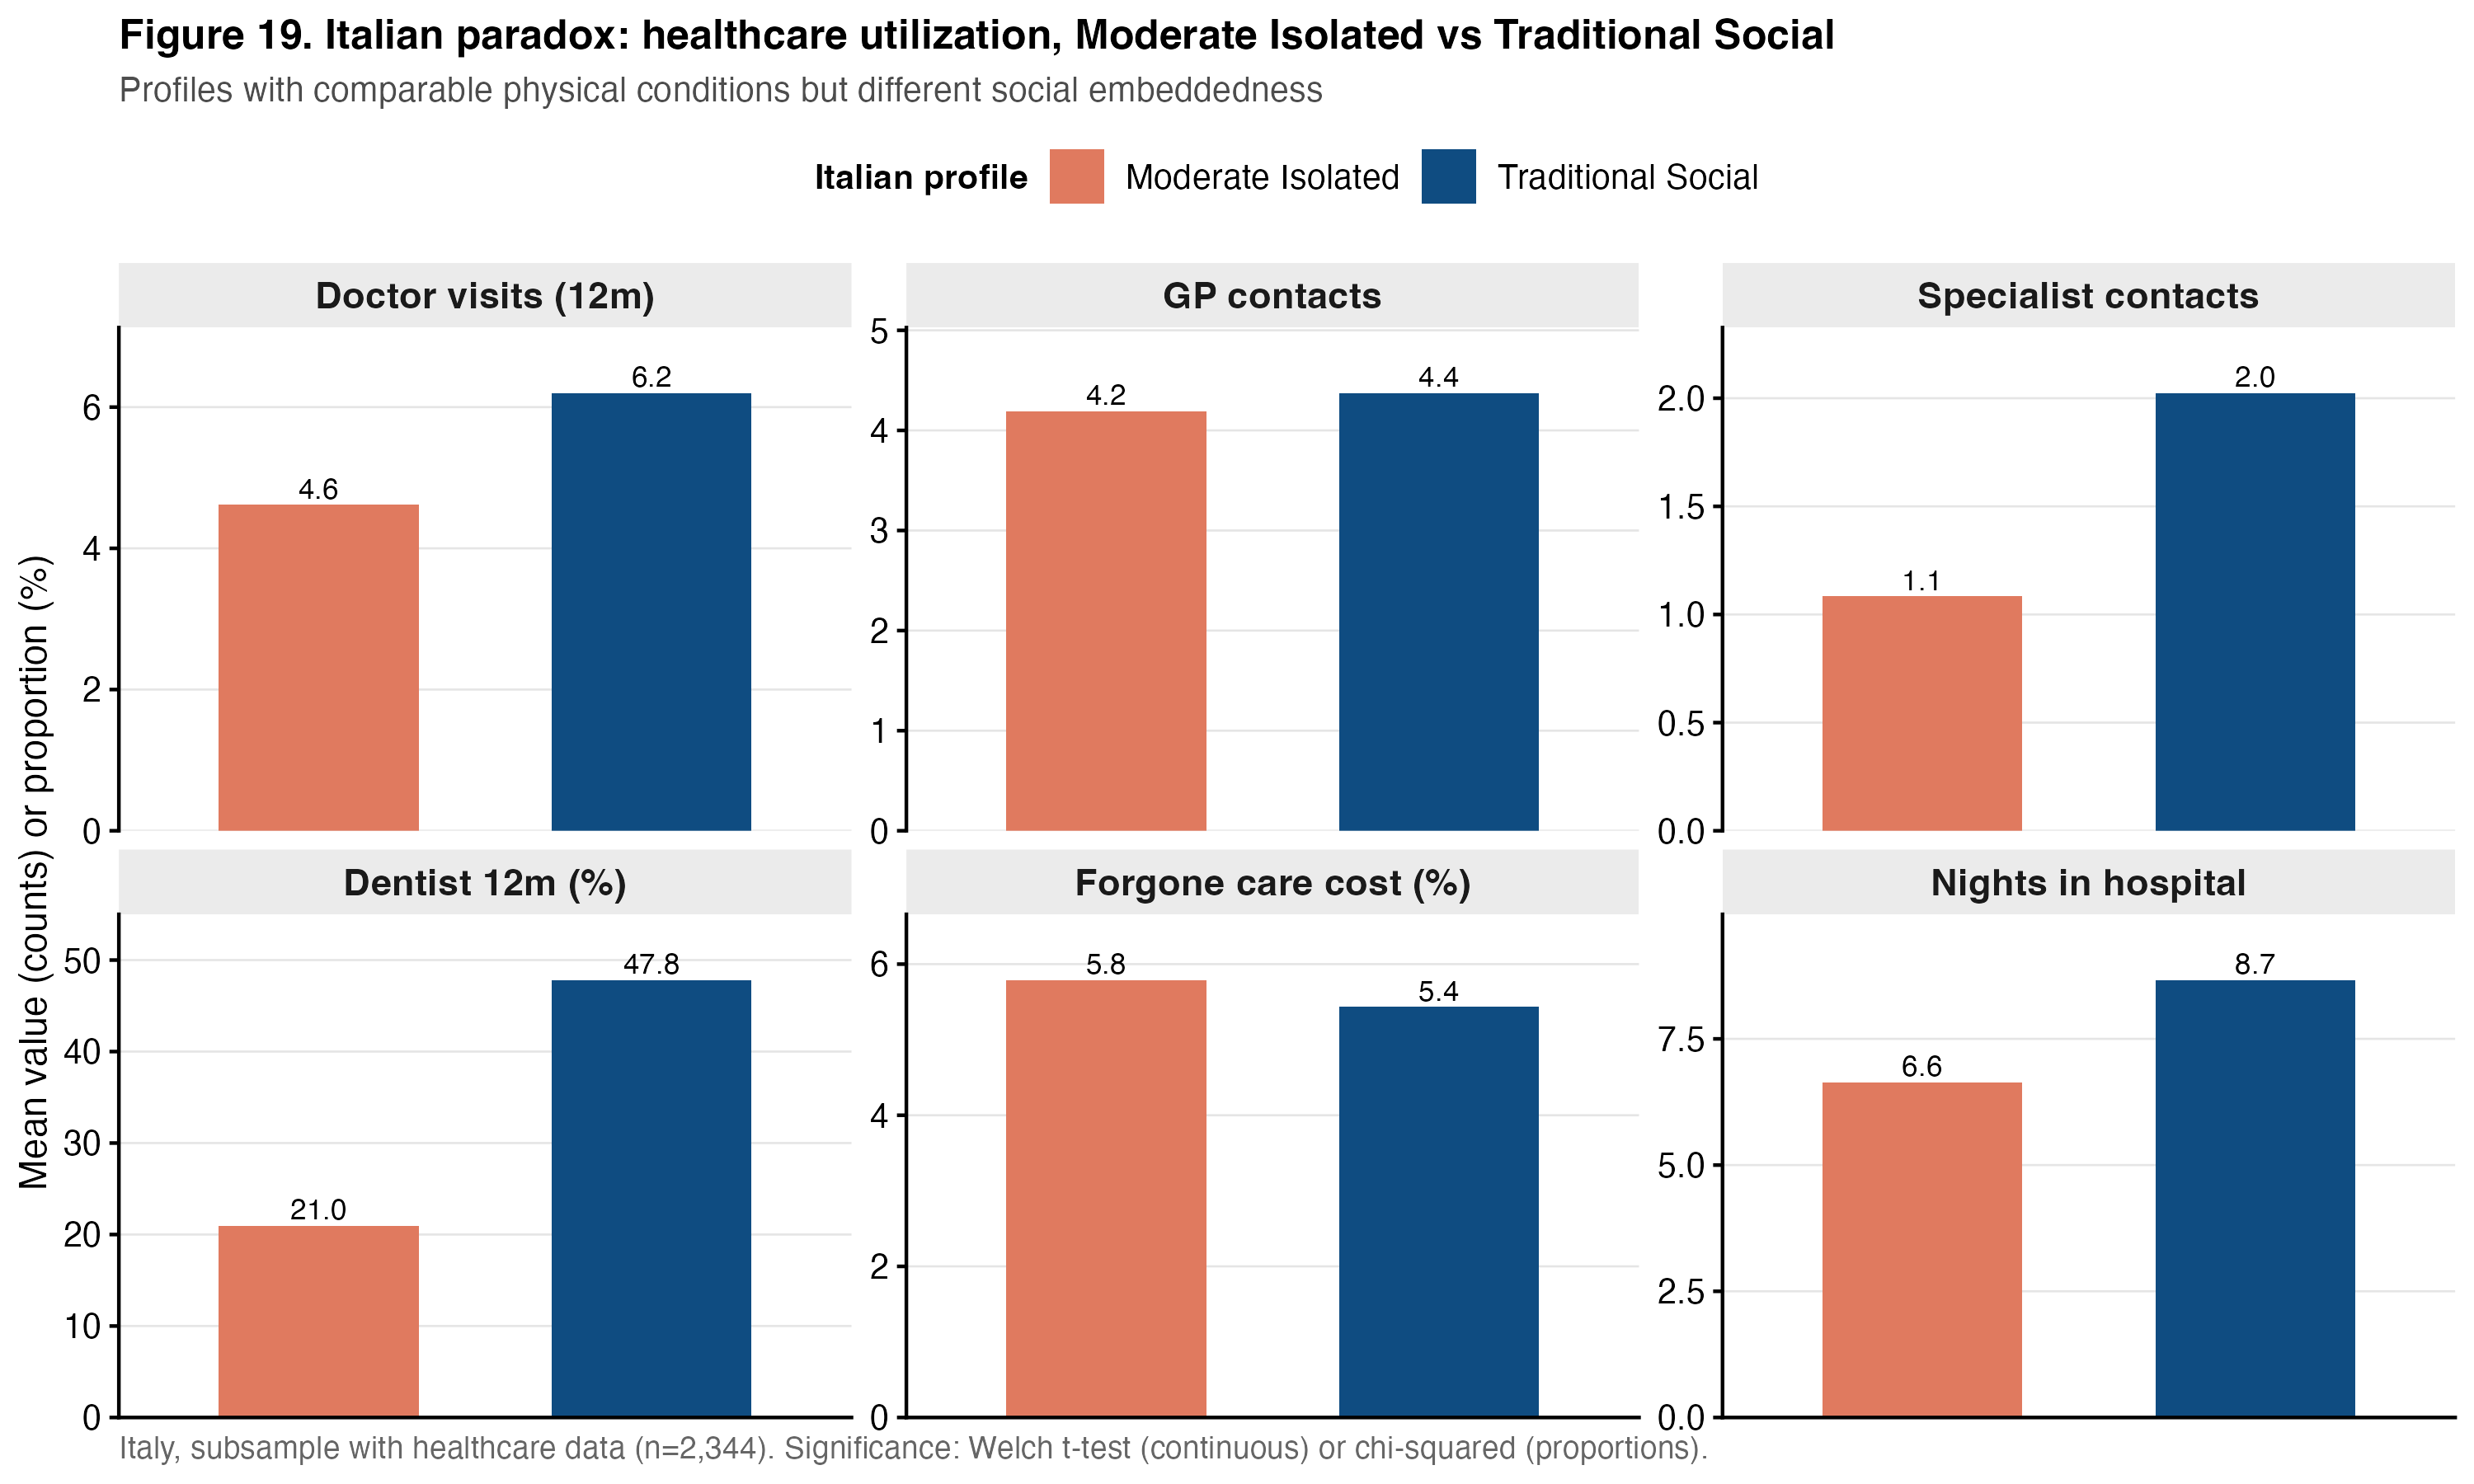
\includegraphics[width=0.92\linewidth]{figures/06_comparison/fig_19_healthcare_italy_isolati_vs_sociali.png}
  \caption{Healthcare indicators by profile: Moderate Isolated vs Traditional Social, Italy. Source: v9 pipeline.}
  \label{fig:ch7-isolati-sociali}
\end{figure}

Three findings emerge. First, on the \emph{prevention-facing} indicators --- doctor visits, specialist contacts, dentist --- the Moderate Isolated profile shows a sharp and highly significant deficit. The dentist gap is the starkest: 21\% of Moderate Isolated respondents saw a dentist in the preceding twelve months, against 48\% of Traditional Social respondents. Doctor visits are 26\% lower in the Isolated group, specialist contacts 47\% lower. Second, on \emph{GP contacts} the gap is essentially zero ($-0.18$, $p = .60$), confirming that the pattern is specific to discretionary interactions with the system and does not extend to the baseline primary-care relationship. Third --- and this is where the v9 estimates revise a preliminary finding from earlier drafts --- the \emph{forgone care for cost} gap is essentially zero ($+0.36$ percentage points, $p = 1.00$) and the \emph{nights-in-hospital} gap is statistically indistinguishable from zero and in the opposite direction ($-2.02$, $p = .47$). Under the current analytical sample, the Moderate Isolated profile does not report more cost-driven forgone care than the Traditional Social profile, nor longer inpatient stays.

\section{Mechanism: navigational capital, not ambulance service}
\label{sec:ch7-mechanism}

The combination of findings in Table~\ref{tab:ch7-isolati-sociali} invites a specific interpretation of the mechanism. A naive reading would posit that the isolated are \emph{unable} to access healthcare because of cost or logistical barriers --- a picture consistent with the forgone-care gap that earlier drafts reported. Under the v9 estimates, that reading is no longer supported: Moderate Isolated and Traditional Social respondents forgo care for cost at equal rates.

The surviving pattern is more specific and, arguably, more informative. Italians with a dense social network take advantage of \emph{discretionary} healthcare services --- the elective specialist visit, the routine dentist appointment, the incremental GP consultation --- at substantially higher rates than Italians without such a network, even when the two groups are indistinguishable on subjective well-being and clinical condition. The difference is not the presence of an acute unmet need that the isolated cannot resolve for lack of money; it is the absence of the incidental social prompting --- the cousin who drives them to the appointment, the neighbour who mentions an exemption, the friend who recommends a reduced-fee provider --- that the Traditional Social profile takes for granted as part of its informal care environment. In this reading, the social network operates as \emph{navigational capital}: a decentralised literacy infrastructure about the system and its affordances, not a volumetric service provider or an economic filter.

This interpretation is consistent with the fact that GP contacts --- the one routine, non-discretionary channel that the Italian system institutionalises (a registered \emph{medico di base} who is expected to be seen at least once a year) --- show no gap, while dentist and specialist visits, which require active initiative, show the largest gaps. The navigational-capital account also explains the null result on forgone care: forgone care for cost captures acute situations in which the respondent \emph{recognises} an unmet need and refrains from addressing it; by contrast, the discretionary-care gap captures situations in which the respondent \emph{does not recognise} the relevant service in the first place.

\section{Cross-country comparison of utilisation}
\label{sec:ch7-crosscountry}

Table~\ref{tab:ch7-crosscountry} reports aggregate utilisation indicators for Italy and Sweden, and Figure~\ref{fig:ch7-cross} visualises the same contrasts.

\begin{table}[ht]
  \centering
  \caption{Aggregate healthcare utilisation, Italy vs Sweden.}
  \label{tab:ch7-crosscountry}
  \small
  \begin{tabular}{@{}lrrrl@{}}
    \toprule
    \textbf{Indicator (12m)} & \textbf{Italy} & \textbf{Sweden} & \textbf{Gap (SE $-$ IT)} & \textbf{$p$}\\
    \midrule
    Doctor visits             &  6.97 &  5.53 & $-1.43$  & $<.001$\\
    GP contacts               &  5.32 &  2.49 & $-2.83$  & $<.001$\\
    Specialist contacts       &  2.10 &  2.06 & $-0.04$  & $.802$\\
    Dentist (\%)              & 30.4  & 83.8  & $+53.4$  & $<.001$\\
    Hospitalised (\%)         &  9.3  & 13.8  & $+4.5$   & $<.001$\\
    Forgone care for cost (\%)& 10.1  &  2.7  & $-7.4$   & $<.001$\\
    Nights in hospital        & 10.92 &  6.18 & $-4.74$  & $.002$\\
    \bottomrule
  \end{tabular}
\end{table}

\begin{figure}[ht]
  \centering
  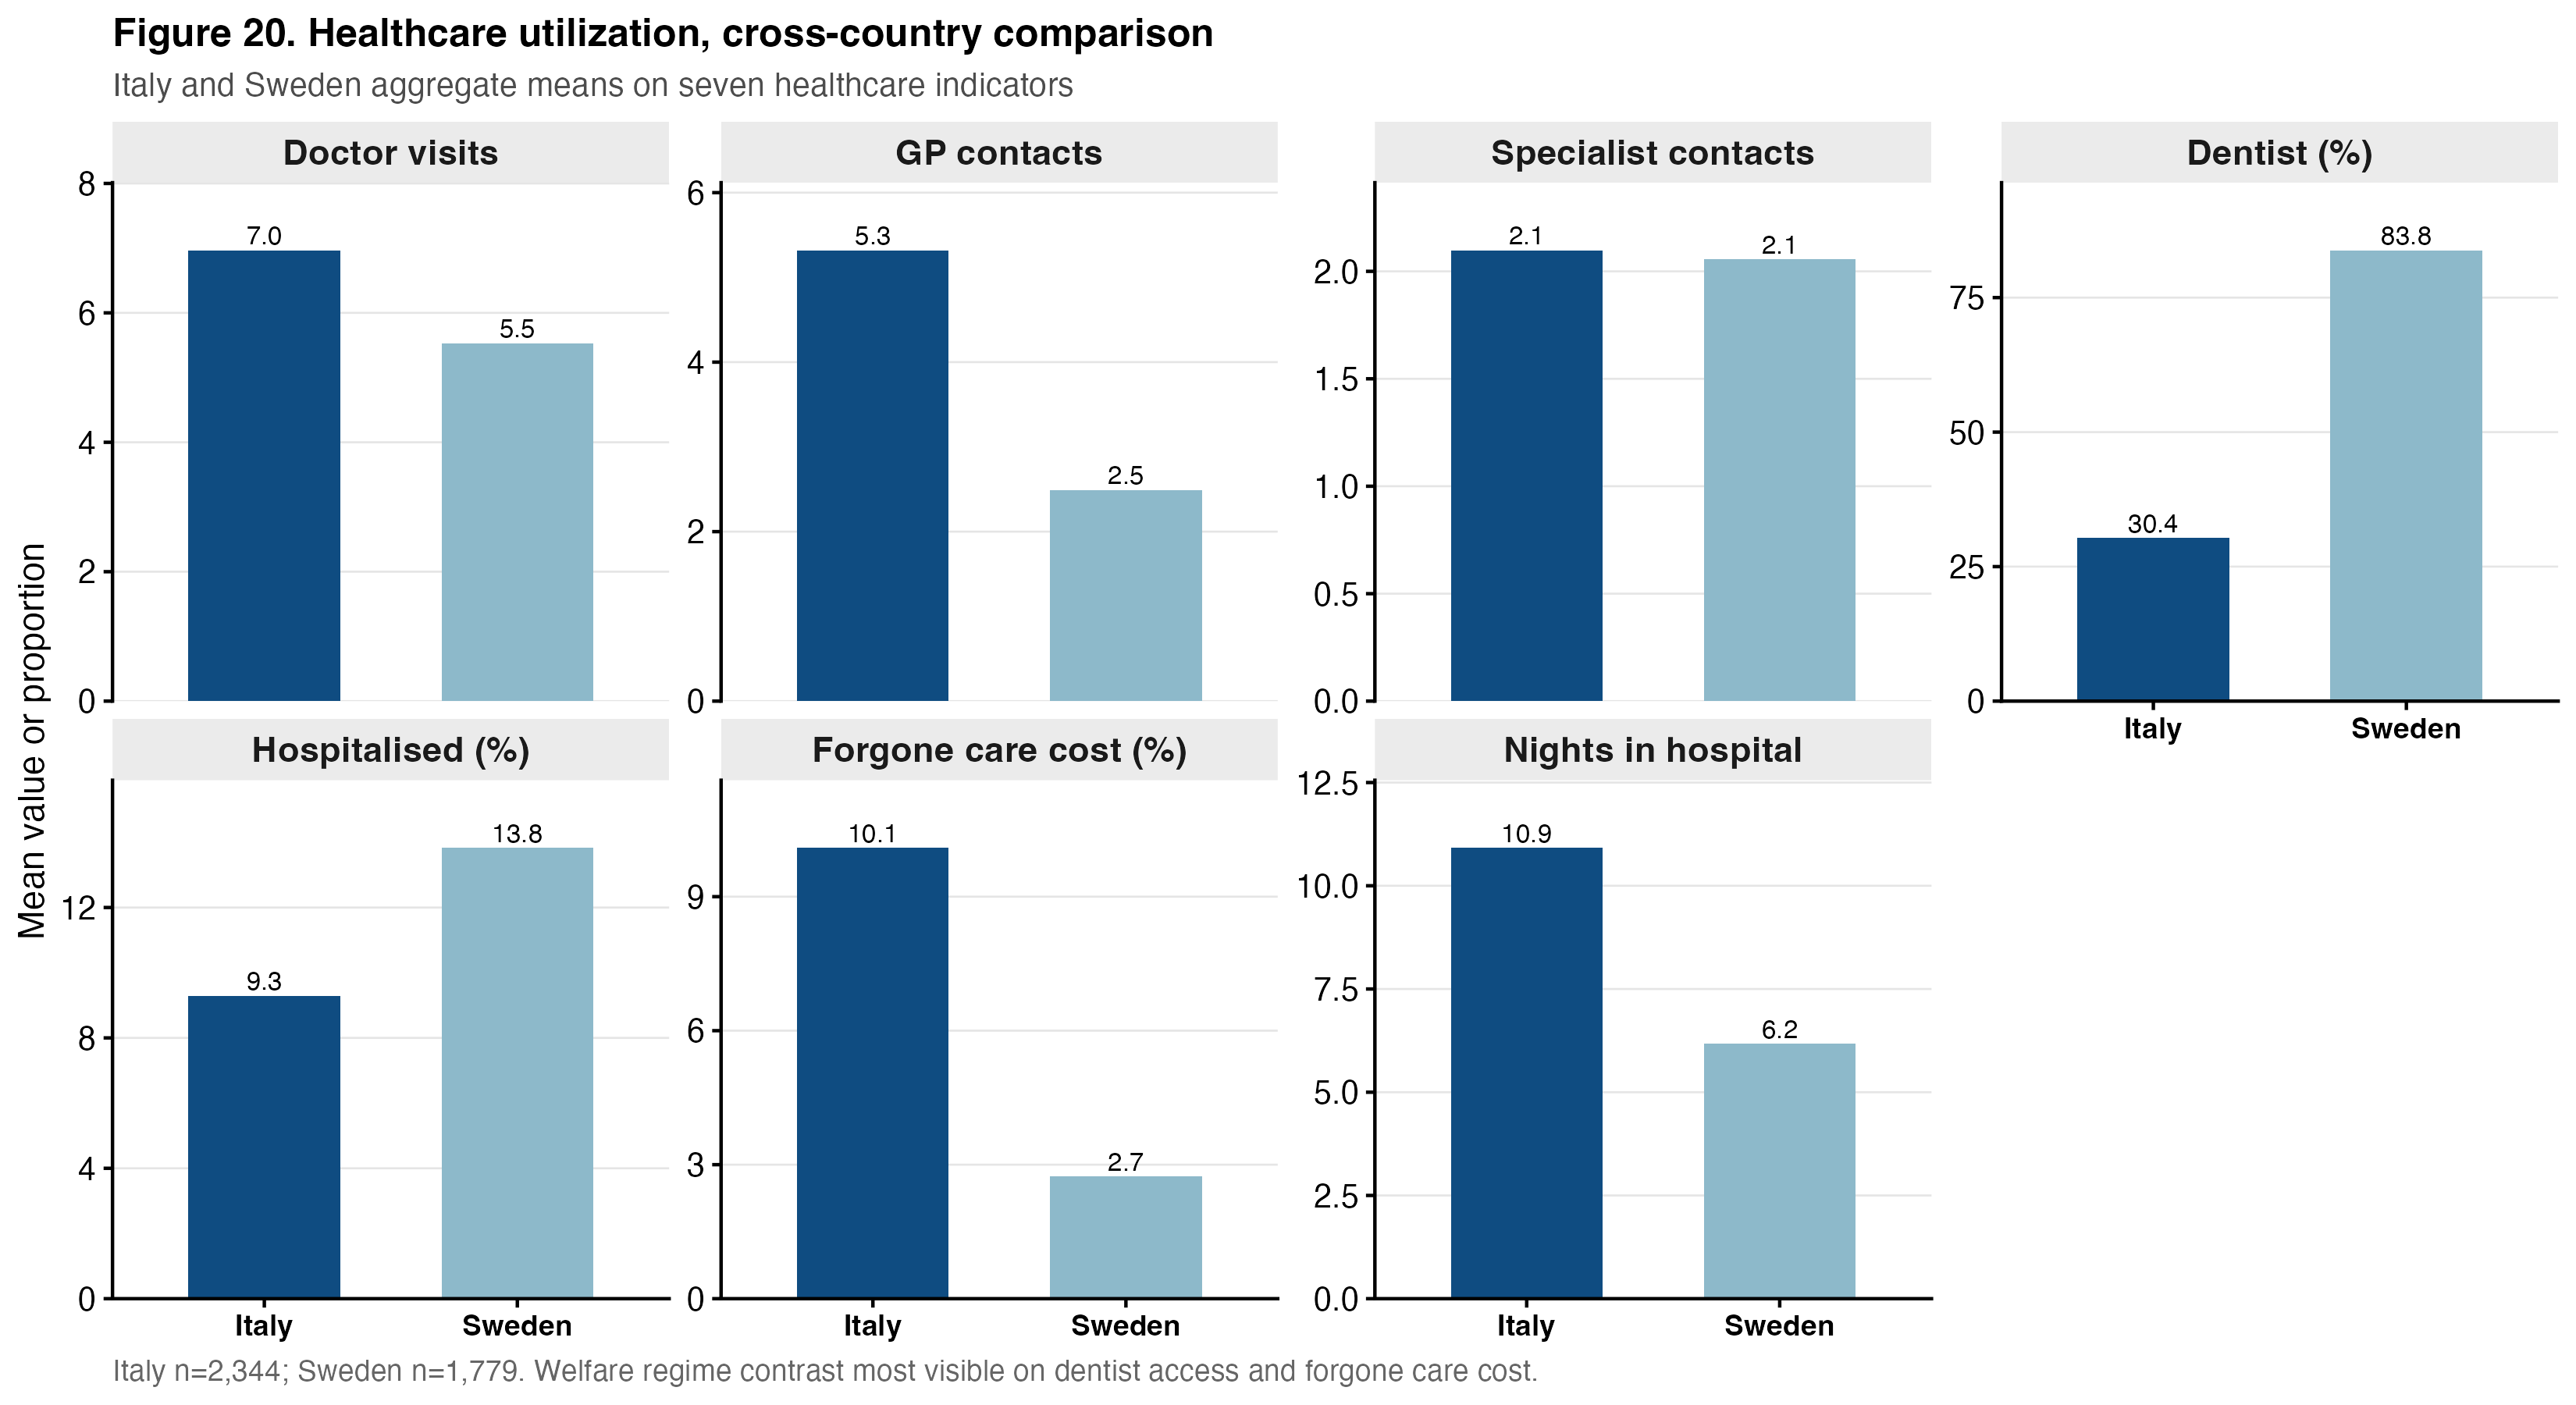
\includegraphics[width=0.88\linewidth]{figures/06_comparison/fig_20_healthcare_cross_country.png}
  \caption{Healthcare utilisation indicators: Italy vs Sweden. Source: v9 pipeline.}
  \label{fig:ch7-cross}
\end{figure}

The cross-country pattern mirrors the within-Italy pattern in a revealing way. Italy exhibits more volumetric contact with the system (more doctor visits, more GP contacts, more and longer inpatient stays) and less \emph{preventive} contact (much lower dentist rate, higher forgone care for cost). Sweden shows the opposite signature: fewer routine contacts, much higher preventive contact, and very low cost-driven forgone care. The welfare-regime contrast is thus legible not only in the profile-level comparison of Chapter~\ref{ch:ch5} but also in the system-level behaviour of the two populations --- with the universalist Swedish system producing a healthcare footprint that is qualitatively different from the Italian familistic one.

\begin{figure}[ht]
  \centering
  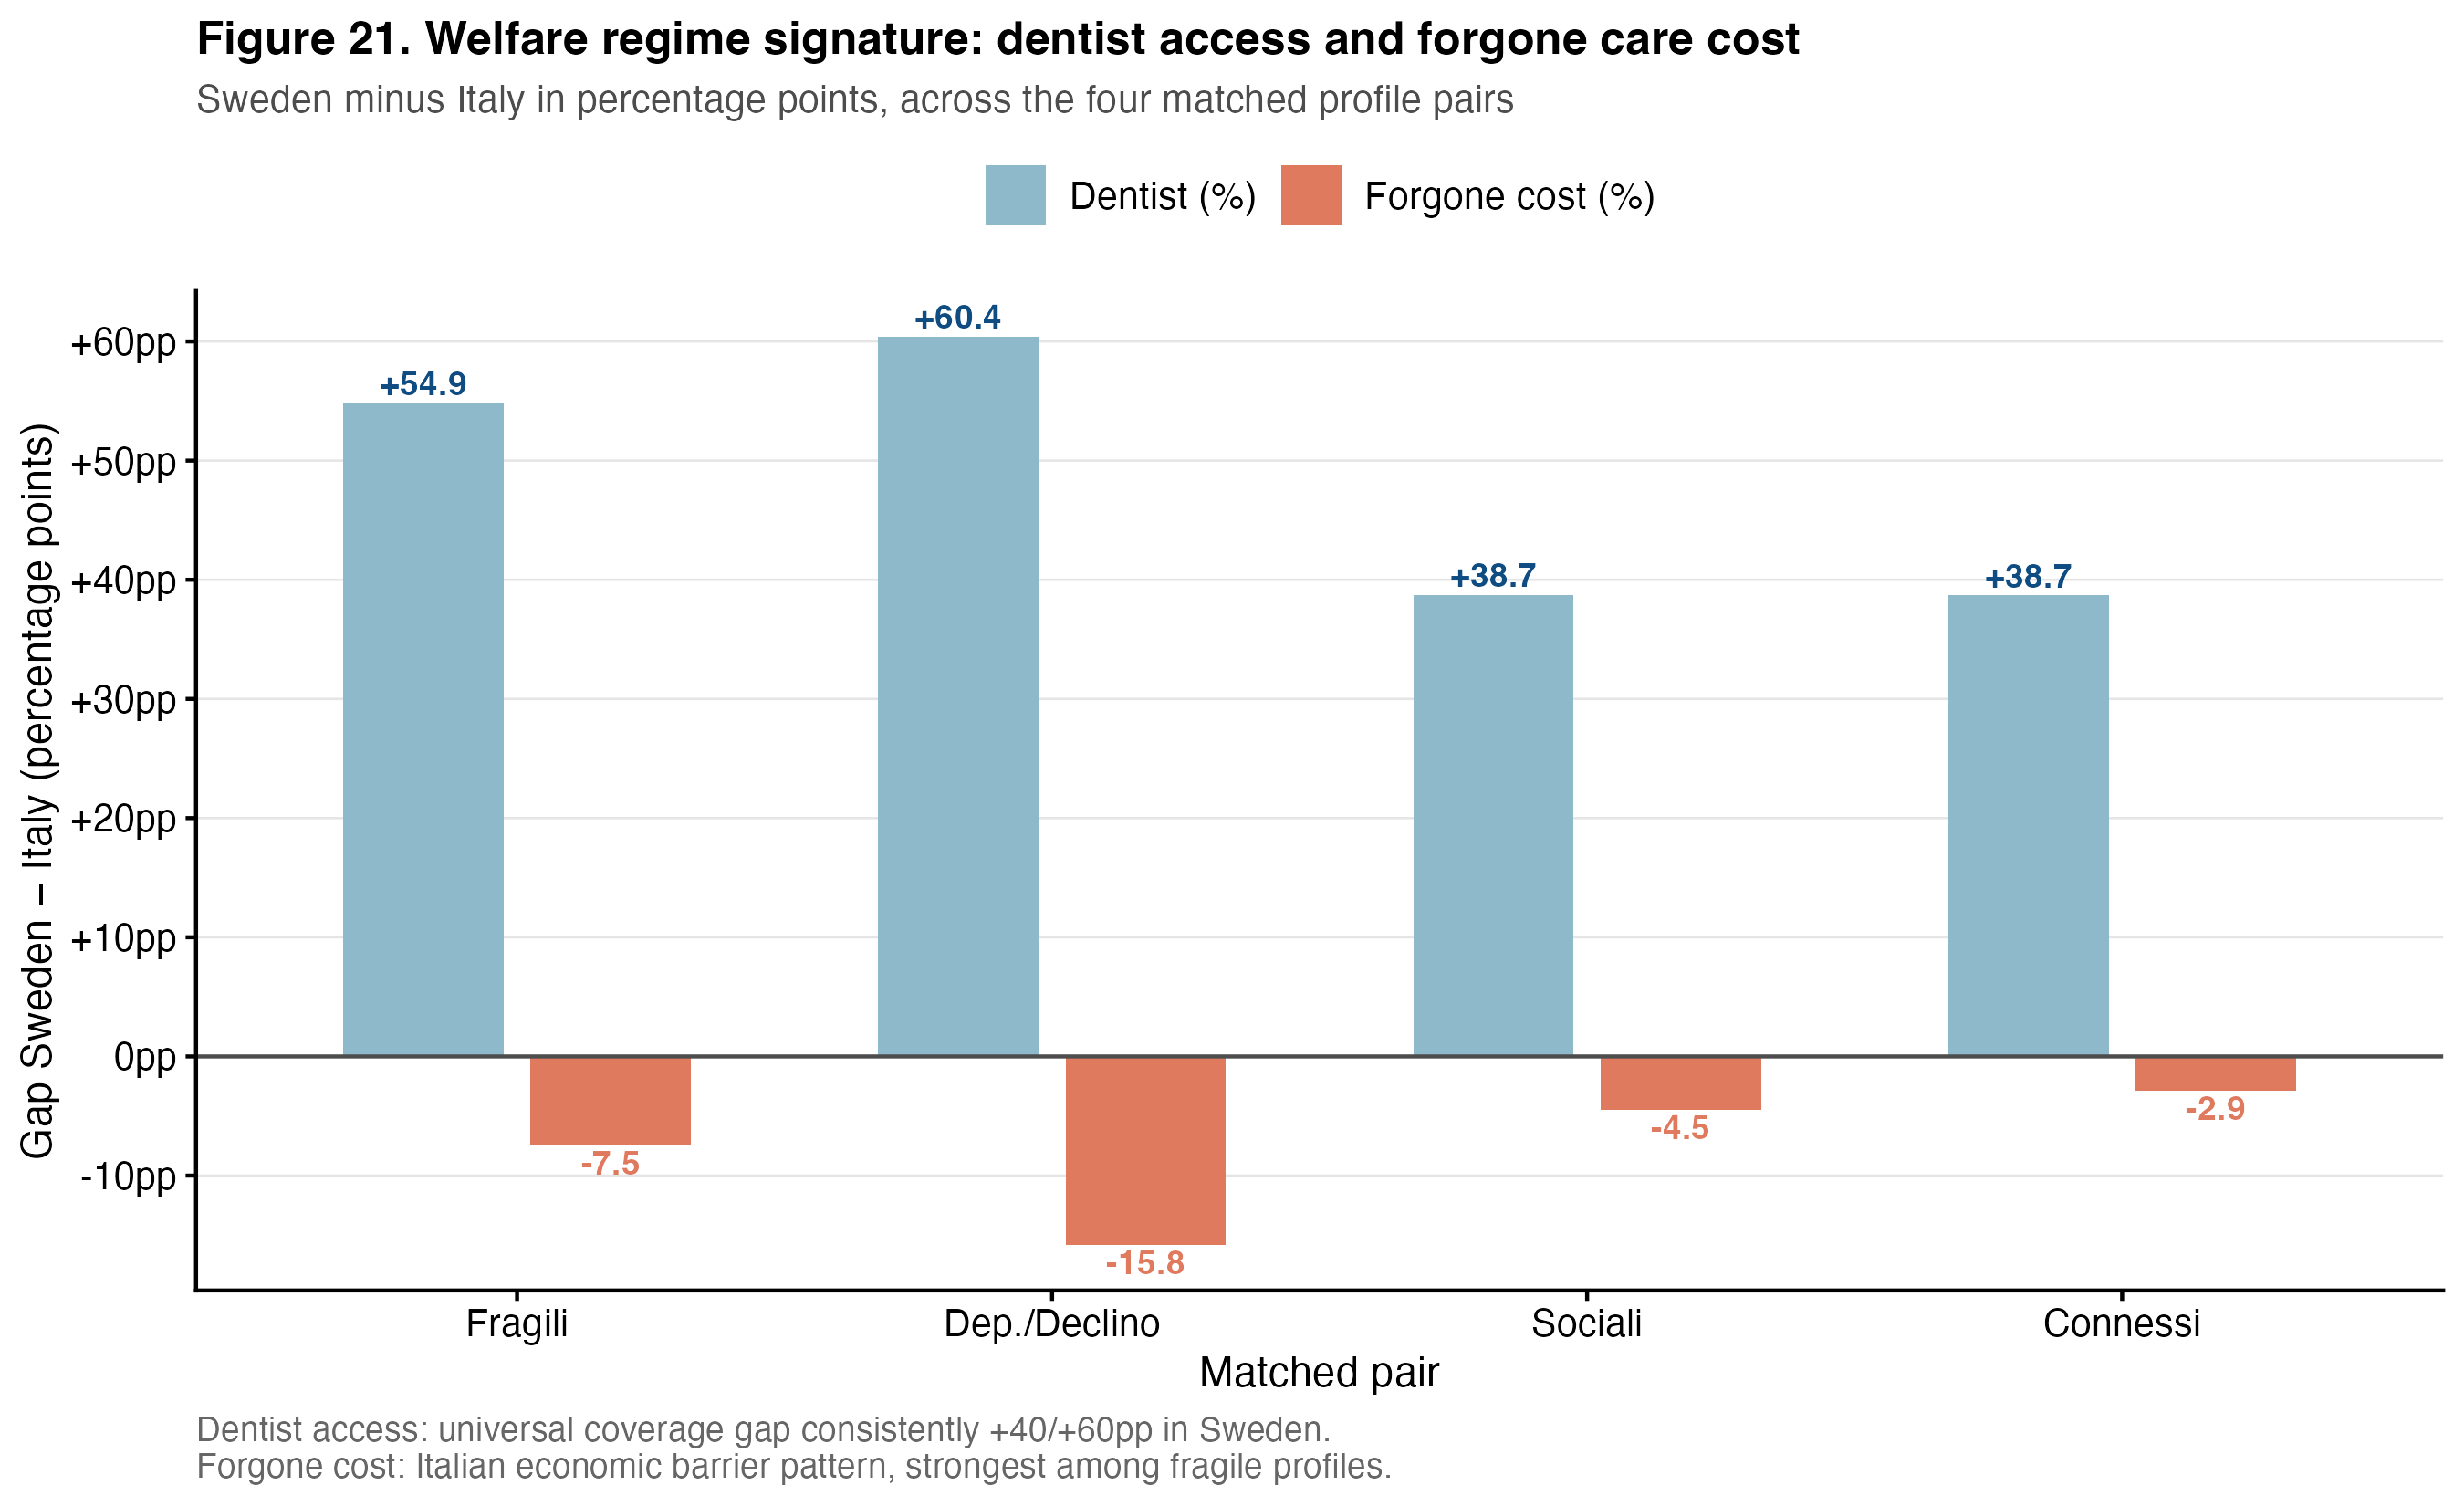
\includegraphics[width=0.78\linewidth]{figures/06_comparison/fig_21_welfare_gap_dentist_forgone.png}
  \caption{Two signatures of the welfare-regime gap: dentist access and forgone care for cost. Source: v9 pipeline.}
  \label{fig:ch7-welfare-gap}
\end{figure}

\section{Chapter summary}
\label{sec:ch7-summary}

The Moderate Isolated profile pays a measurable cost for invisibility: it uses discretionary healthcare services at sharply lower rates than the matched Traditional Social profile under comparable clinical conditions. The pattern is specific to services that require active initiative (specialist, dentist) and does not extend to the routine GP channel. Forgone care for cost, however, does not differ between the two groups, which rules out an economic-barrier reading and points instead to a navigational-capital mechanism: the social network helps its members \emph{discover} and \emph{enact} entitlements, not \emph{afford} them. The cross-country comparison is consistent: Italy as a whole shows the same preventive-deficit / volumetric-excess signature that distinguishes the Moderate Isolated from the Traditional Social within Italy. Chapter~\ref{ch:ch8} draws the policy implications.
